\documentclass{article}
\usepackage[english]{babel}
\usepackage[letterpaper,top=2cm,bottom=2cm,left=3cm,right=3cm,marginparwidth=1.75cm]{geometry}
\usepackage{amsmath, graphicx, authblk, fullpage, apacite}
\usepackage{natbib}
\usepackage[colorlinks=true, linkcolor=black, citecolor=black, urlcolor=blue]{hyperref}



\title{Capstone Project Literature Review: Yelp Sentiment Analysis}
\author{Joshua Aflleje}
\author{Nicole Feil}
\author{Andrew Liu}
\author{Jack Oebker}
\affil{Arizona State University, Tempe, AZ 85281, USA}

\begin{document}
\maketitle

\section{Introduction}
Online reviews play a crucial role in shaping consumer behavior and business success. Platforms like Yelp, Google Reviews, and TripAdvisor significantly influence purchasing decisions. \citep{reviewtrackers2025} states that approximately 92.4\% of customers rely on online reviews to guide most of their purchasing decisions, and around 63.6\% of consumers read reviews before visiting a business. Among these platforms, Yelp is one of the most influential review platforms. 

Yelp, a prominent online review platform, hosts millions of user-generated opinions covering restaurants, healthcare providers, and a wide range of local businesses. These reviews provide valuable insights for both consumers and business owners, shaping purchasing behavior and informing service improvements. However, while numerical star ratings offer a quick reference point, they often fail to capture the depth and nuances of consumer sentiment. Yelp’s star rating system reduces potentially complex reviews into single numerical values. A five-star rating may indicate general satisfaction, but it does not differentiate which factors in particular contributed to it. 

Recent advances in sentiment analysis have attempted to bridge this gap by moving beyond simple sentiment classification to more granular, aspect-based approaches. Researchers now aim to extract actionable insights by identifying specific features—such as food taste, service quality, and ambiance—that influence positive or negative feedback \citep{HuLiu2004}. This transition toward aspect-based sentiment analysis (ABSA) has enabled businesses and researchers to obtain a more detailed understanding of customer experiences.

As sentiment analysis techniques have grown more advanced, researchers have identified key challenges such as data biases and review authenticity. Studies such as \cite{Liang2018} have demonstrated how NLP models can predict Yelp ratings based on review text, while \cite{Mukherjee2021} have explored the impact of fake reviews and how they distort sentiment analysis outcomes. Studies have shown that Yelp’s filtering algorithm disproportionately flags extreme sentiment reviews—whether genuine or not—introducing bias into overall ratings \cite{Mukherjee2021}.

\subsection{Background}

Sentiment analysis initially focused on classifying entire reviews as positive or negative, oversimplifying consumer feedback, particularly for products and services where different aspects could receive distinct evaluations.

However, \cite{HuLiu2004} introduced aspect based sentiment analysis (ABSA), which identifies specific product or service attributes and evaluates their associated sentiment. Their research involved identifying opinion words (e.g., ”delicious,” ”expensive,” ”friendly”) and linking them to corresponding features (e.g., ”food,” ”price,” ”service”). Aspect-based sentiment analysis has since been widely used to enable businesses to understand which aspects drive customer satisfaction or dissatisfaction and to allow them to target improvements.

Although Yelp is most commonly associated with restaurant reviews, its influence extends to non food-related businesses, including healthcare. \cite{ChenLee2024} examined how Yelp ratings impact physician selection, demonstrating that sentiment-laden text in reviews significantly influences patient decision-making. \cite{ChenLee2024} analyzed Yelp physician reviews and found that sentiment strongly influences patient choice. Their research showed that a one-star increase in rating resulted in a 1.9\% revenue increase and a 1.2\% rise in patient volume \citep{ChenLee2024}. This highlights the real-world impact of sentiment analysis beyond restaurants, making it applicable to professional services where interpersonal interactions shape consumer decisions. It also suggests that businesses in diverse industries can benefit from opinion mining to improve customer engagement and service quality.

\cite{KellerKostromitina2020} explored how non-chain restaurants are rated on Yelp, differentiating them from larger franchise operations. Their study analyzed thousands of Yelp reviews to uncover key factors that influence star ratings such as independent restaurants being more likely to be judged on their uniqueness and atmosphere. Their findings emphasize the importance of contextualizing sentiment analysis models based on business type because factors influencing ratings can vary significantly between independent and chain restaurants. 

\cite{Liang2018} examined how machine learning models can predict Yelp ratings based on sentiment and topic models. The study employed natural language processing (NLP) techniques to analyze review text and infer numerical ratings, demonstrating the feasibility of automated review classification. By using topic modeling approaches such as Latent Dirichlet Allocation (LDA), Liang’s study identified hidden themes in Yelp reviews and mapped them to sentiment scores, highlighting how computational methods can enhance traditional sentiment analysis.

\section{Methodologies}

\subsection{Aspect-Based Sentiment Analysis (ABSA)}
Aspect-based sentiment analysis (ABSA) provides a structured approach to extracting important features from Yelp reviews and assigning sentiment labels to those aspects \citep{HuLiu2004}. Deep learning techniques, such as BERT-based transformers, have significantly enhanced ABSA performance. The integration of multi-layered graph convolutional networks (GCNs) with BERT can allow for more effective sentiment dissection by capturing complex relationships between aspects within a review \citep{Aziz2024}. The approach combining aspect-specific embeddings with sentiment propagation across review structures leads to a nuanced understanding of user opinions \citep{Aziz2024}.

\begin{figure}[h]
    \centering
    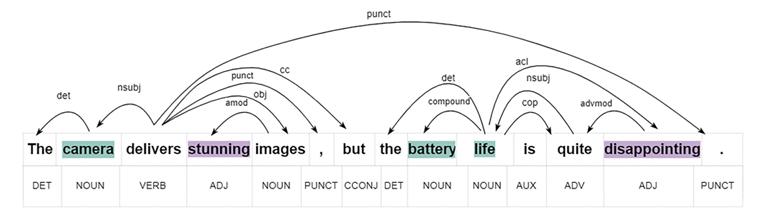
\includegraphics[width=1.0\textwidth]{absa.png} % Places absa picture
    \caption{Diagram depicting the process of ABSA}
    \label{fig:myimage}
\end{figure}
\begin{center}
Source: \cite{Aziz2024}
\end{center}

\subsection{Sentiment-Driven Business Recommendations}
Currently, Yelp suggests businesses based on categories and location, without factoring in sentiment-driven preferences. Clustering businesses based on user sentiment trends can offer a more personalized recommendation system \citep{KellerKostromitina2020}. This can be achieved using vector-based similarity models, which compare businesses based on review sentiment patterns rather than just business type. By leveraging sentiment-driven clustering techniques, businesses can be grouped based on their perceived strengths and weaknesses, providing users with more tailored recommendations.

\subsection{Synthetic Review Generation}
Generative models, such as GPT-based architectures, can create synthetic reviews at different star levels by leveraging sentiment analysis. These synthetic reviews, conditioned on real sentiment trends, provide users with a summarized representation of a business’s strengths and weaknesses without manually reading thousands of reviews. By integrating this methodology with Sentiment-Driven Business Recommendations, we can generate representative reviews based on a business's star rating using a predefined word bank. This approach allows us to predict how future customer reviews might appear given the business’s overall sentiment distribution and rating trends.

\section{Conclusion}

Sentiment analysis of Yelp reviews has evolved from simple star-based evaluations to more nuanced aspect-based sentiment analysis (ABSA), enabling businesses to better understand customer experiences. Studies have demonstrated that sentiment in reviews significantly influences consumer decisions across industries, from restaurants to healthcare \citep{HuLiu2004, ChenLee2024}. However, challenges remain, including biases in Yelp’s filtering algorithms and the impact of fake reviews \citep{Mukherjee2021}. Advanced methodologies, such as deep learning and generative models, offer promising solutions for improving sentiment classification and business recommendations \citep{Aziz2024}. Furthermore, synthetic review generation based on sentiment trends provides a novel approach for summarizing business reputations and predicting potential reviews, enhancing consumer insights. As sentiment analysis techniques continue to advance, their applications will expand, providing more precise and personalized insights for businesses and consumers alike.

\newpage
\bibliographystyle{apalike}
\nocite{*}
\bibliography{ref}

\end{document}